\section{\AVOIRmethodname{} Framework}
\subsection{Definitions}
\begin{table}
    \centering
    \small
    \begin{tabular}{cl}
        \toprule
         \textbf{Symbol} &  \textbf{Description} \\
         \midrule
         $\Delta$ & Overall failure probability for a specificaiton \\
         $X_i$ & Bernoulli random variable for $i^{tg}$ tern\\
         $\BarE[X]$ & Empirical estimate of expectation $\E[X]$\\
         $t$ & No. of observed samples \\
         $\BarE[X_i]_t$ & Empirical estimate after $t$ steos  \\
         $\delta_i$ & Failure probability $0 \leq \delta_i \leq 1$ corresponding  to $X_i$ \\
         $\varepsilon_i$ & Concetration bound for $|E[X_i] - \BarE[X_i]| \leq \varepsilon_i$ \\
         $\phi_X$  & Concentration bound for empirical estimate of $E[X]$ \\
         $\psi$ & Fairness specification\\
         $r, R$ & Return value of the function being monitored\\
         $y, Y$ & True label \\
         $s, S$ & Indicator for group membership \\
         $c$ &  Constant $\in \R$ \\
         $C$ & A set of constraints\\
         \bottomrule
    \end{tabular}%
    \caption{The \AVOIRmethodname{} symbol descriptions table.}
    \label{tab:definitions}
\end{table}
\AVOIRmethodname{} supports implementing an extensive range of group fairness criteria, including demographic parity~\citep{calders2009building}, equal opportunity~\citep{hardt2016equality}, disparate mistreatment~\citep{zafar2017fairness}, and combinations of these criteria. 
For instance the above 80\%-rule is \lstinline{E[r|S==s]/E[r|S!=s] > 0.8} in \AVOIRmethodname{}'s DSL\footnote{Domain Specific Language}.
Here, the term \lstinline{E[r|S==s]/E[r|S!=s]} is a \textit{subexpression} of the specification.
The smallest units involving an expectation (e.g., \lstinline{E[r|S!=s]}) are denoted as \textit{elementary subexpressions}.
We focus on fairness criteria that can be expressed using Bernoulli r.v. as it allows the simplification of probabilities into expectation, as $\Pr[r = 1] = \E[r]$ (hereafter, used interchangably).
Our algorithm uses adaptive concentration sets~\citep{zhao2016adaptive,howard2021time} to build estimates for \textit{elementary subexpressions} and then derive the estimates for expressions that combine them.
A combination of multiple such elementary expressions is denoted as a \textit{compound} expression.
We aim to derive statistical guarantees about fairness criteria based on estimates from observed inputs and outputs.
For example, let $X$ be an observed Bernoulli r.v, then an assertion $\phi_X = (\BarE[X], \epsilon, \delta)$ over $X$, corresponds to an estimate satisfying $\phi_X \eqdef \Pr[|\E[X] - \BarE[X]| \geq \epsilon] \leq \delta $
where $\BarE[X]$ denotes an empirical estimate of $E[X]$.
We then use assertions $\phi_X, \phi_Y$ to assert claims for expressions involving $X, Y$.
For example, for the 80\%-rule, assertions over $\E[X]/\E[Y]$.
A \textit{specification} involves either a comparison of expressions with constants (e.g., $\E[X]/\E[Y] > 0.8$) or combinations of multiple such comparisons. 
Such a specification may be True ($T$) or False ($F$) with some probability.
For a given specification $\psi$, we denote the claim that $P[\psi = F] \geq 1 - \Delta$ as $\psi: (F, \Delta)$, where $\Delta$ denotes the failure probability of a guarantee. 
Given a stream of observations and outcomes from the decision functions, and a specified threshold probability $\Delta$, we will continue to refine the estimate for a given specification until we reach the threshold.
Specifications involving variables that take more than two values can be implemented using transformations and boolean operators (examples in Appendix~\ref{sec:appendix:additional-metrics}).

\subsection{Language Specification}
\label{sec:theoretical:specification}

\begin{figure}
    \centering
    %\begin{grammar}
             <spec> ::= <ETerm>  <comp-op>  c 
                \alt <spec> $\land$ <spec>              
                \alt <spec> $\lor$ <spec> 
        
            <ETerm> ::= $\E[<E>]$
                \alt   $\E[<E>$|$<E>]$
                \alt   c $\in \R$
                \alt   <ETerm> $\ \{+, -, \times, \div \}\ $ <ETerm>
\end{grammar}
    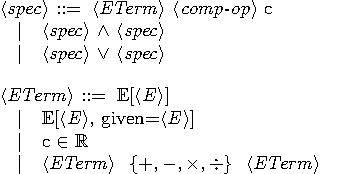
\includegraphics{avoir/images/grammar}
    \caption{Grammar for specification. $\langle E \rangle$ refers to  expressions of r.vs and $\langle comp-op \rangle = $ comparison operator $\in \{>, <, =, \neq\}$.}
    \label{fig:grammar}
\end{figure}
We describe \AVOIRmethodname{}'s DSL used for specifying fairness metrics (\Cref{fig:grammar}).
We focus on binary decision-making functions; Bernoulli r.v.s can characterize their outputs.
%Note that for such a Bernoulli r.v. $X$, $\E[X] = \Pr[X = 1]$ and hereafter, these are used interchangeably. 
Consider a decision function $f: X \rightarrow \{0, 1\}$, where $X = (X_1, \dots, X_k)$ denotes a real-valued input vector. 
We use $R = f(X)$ to simplify the remainder of the definitions. 
The grammar can be used to construct Bernoulli r.vs to support expressions beyond those that produce binary outputs.
For example, a $\nu$-threshold based real-valued output, $R' = (R > \nu)$ and a multi-class output, for class $j$,  $R' = (R == j)$ correspond to Bernoulli r.vs.
Expressions involving $R$ and $X_i$ act as the arguments \lstinline{<E>} to construct an \lstinline{<ETerm>}.
For example, $\E[R > 0 | X_1 + X_2 > a]$.
$c$ terms represent constant real values used as bounds for specifications.
We modified the grammar from prior work to include two additional operations. 
First, we added a \texttt{given} argument to $\E$, which allows a user to specify conditional probabilities directly, in contrast to specifying it as a ratio of joint/marginal probabilities. 
 \begin{align*}
     \frac{\E(A \vee (B=b))}{\E(B=b)} \rightarrow \E(A, \mathtt{given}=(B=b))
 \end{align*}
 which is used to represent $\E[A|B=b]$, simplifying expressions for group fairness specification.
Additionally, we add comparison operators, which further simplify the process of writing specifications. 

\subsection{Propagating Bounds}
\label{sec:theoretical:propagation}
%\paragraph{Inference and Optimization}
Generating the bounds for a specification requires propagating them from elementary subexpressions.
Assuming that observed values for each \texttt{<E>} correspond to an underlying random variable $X$,
a probabilistic guarantee $\phi_X$ for an \textit{elementary} subexpression consists of an empirical estimate $\BarE[X]$, a concentration bound $\epsilon_X$, and a failure probability $\delta_X$, such that $\Pr[|\E[X] - \BarE[X]|\geq \epsilon_X] \leq \delta_X$.
For compound expressions, we must infer the implied guarantees that can be inferred with corresponding constraints.
%In addition, guarantees may require certain constraints to be satisfied.
Each inference rule corresponds to a derivation in the DSL grammar.
Inference rules have preconditions and postconditions that are in the form:
\begin{align*}
 \frac{\bigcup \left\{r | r \in \{\phi, \psi, C \}\right\}}{\bigcup \left\{s | s \in \{ \phi, \psi, C \} \right\} }
\end{align*}
where $\phi$ denotes a claim for a subexpression, $\psi$ for a \verb|<spec>|.%, $\BarE$ and $\epsilon$ are the mean and concentration terms associated with a subexpression claim,  $C$ denotes a constraint. 
For example, consider the sum/difference rule. 
Starting with the assumptions $\phi_X \eqdef (\BarE[X], \epsilon_X, \delta_X)$, $\phi_Y \eqdef (\BarE[Y], \epsilon_Y, \delta_Y)$.
Then we have
\begin{align*}
    |\E[X] \pm  \E[Y] &- (\BarE[X] \pm \BarE[Y])| \\
                      %&= |(\E[X] - \BarE[X]) \pm  (\E[Y] - \BarE[Y])| \\
                      & \leq |\E[X] - \BarE[X]| + |\E[Y] - \BarE[Y]|\\
                      & \leq \epsilon_X + \epsilon_Y
\end{align*}
i.e., $\phi_X, \phi_Y \Rightarrow X \pm Y: \left(\BarE[X] \pm \BarE[Y], \epsilon_X + \epsilon_Y, \delta_X + \delta_Y\right)$.
Inference rules may require constraints, for e.g., assume $\phi_X \eqdef (\BarE[X], \epsilon_X, \delta_X)$, $\BarE[X] > c$. 
Then we have $\Pr[\E[X] < \BarE[X] - \epsilon_X] > 1 - \delta$
If we add the constraint that $\BarE[X] - \epsilon_X \geq c$, we have $\Pr[X < c] > 1 - \delta$, thus, 
\begin{align*}
    \phi_X \Rightarrow \psi \eqdef X > c: (T, \delta_X) \\
    \text{under the constraint } \{ \BarE[X] - \epsilon_X \geq c\}
\end{align*}
The complete set of inference rules required for the DSL is provided in the appendix (\Figref{fig:inference}).
The implementation in \AVOIRmethodname{} follows these rules but could be extended to other rule inference templates that support the DSL.
Note that these rules extend the ones implemented by VF~\citep{bastani2019probabilistic} with constraints that enable the optimizations required in \AVOIRmethodname{}. 




\subsection{Optimizing Bounds}
\label{sec:theoretical:optimization}


\subsubsection{\AVOIRmethodname{} Algorithm}
\label{sec:implementation}
\begin{algorithm}
    \caption{\AVOIRmethodname{} Algorithm}
    \label{alg:method}
    \small
    \begin{algorithmic}[1] % The number tells where the line numbering should start
        \Require $\Delta$, $\psi$ \Comment{$\Delta$, Specification} 
        \Ensure $T_s$ time step when the value of $\psi$ can be guaranteed with probability $ \geq 1 - \Delta$
        \For{$X_i \in \psi $}
            \State $\delta_{X_i} = \Delta$ \Comment{Set initial value $\forall i$}
            \State $S_{X_i} = 0$ \Comment{Sum of observations}
            \State $n_{X_i} = 0$ \Comment{Number of observations}
        \EndFor
        \State $T = 0$ \Comment{Time step}
        %\State Initialize $N$ as the number of $E$ terms in $\psi$
        \State Initialize $OPT_\psi$ \Comment{Initialize Optimization Problem (Fig.~\ref{fig:inference})}
        \Procedure{Observe}{$X$} 
            \For{$X_i \in X$}
                \State $S_{X_i} = S_{X_i} + X_i$
                \State $n_{X_i} = n_{X_i} + 1$
                \State $\BarE[X_i] = S_{X_i}/n_{X_i}$
                \State Initialize $\delta_{X_i}$ as a symbolic variable
                \State Assign $\epsilon(\delta_{X_i}, n_{X_i})$ symbolic variable
            \EndFor
            \State Propagate $\delta_{X_i}$ using the inference rules
            \State Initialize constraints $g_K$ in $OPT_\psi$ using the computed values
            \State $\delta^*_T = \texttt{Solve}(OPT_\psi)$
            \If{$\delta^*_T \leq \Delta$}
                \State $\delta_{X_i} = \delta^*_T[X_i]$ 
                \State \Return $T_s = T$
            \EndIf
            \State $T = T + 1$
        \EndProcedure
    \end{algorithmic}
\end{algorithm}
The pseudocode for the optimization procedure in \AVOIRmethodname{} is described in Algorithm~\ref{alg:method}.
The input to the algorithm is the reporting threshold probability $\Delta$ and a specification $\psi$.
We then infer a symbolic optimization problem corresponding to the bounds and failure probabilities of the elementary subexpressions.
At each step, the \texttt{OBSERVE(X)} function is called with the new observation of every elementary subexpression and output.
The empirical running means and counts of observations are updated.
The final optimization problem \texttt{OPT} corresponding to each specification is a nonlinear constrained optimization problem.
If a solution is successfully found for \texttt{OPT}, the algorithm terminates, and the estimate for the specification has reached the required threshold.
If no solution is found, the estimates will be updated with $\delta_i = \Delta$ for each \textit{elementary} subexpression.
The intuition behind the algorithm is to use a confidence sequence corresponding to the estimates of elementary subexpressions at each time step.
The inferred \texttt{OPT} has the form
\begin{align}
    \label{eq:optimization}
    \begin{split}
        &\min_{0 \leq \delta_i \leq 1} \sum_{i=1}^{n}\delta_i  \\
        \text{s.t. } &g_k(\delta_{1, \dots, n}, \BarE[X_1], \dots, \BarE[X_n]) \leq \epsilon_k\\
        %& 0 \leq \delta_i \leq 1
    \end{split}
\end{align}
where $g_k, \epsilon_k$ are the functions/bounds derived using the transformations carried out through the inference rules (Appendix~\ref{sec:appendix:inferrence-rules:opt}).

\begin{definition}
For $\delta \in [0, 1]$, a $1-\delta$ \textit{confidence sequence} is a sequence of confidence sets, usually intervals  $(\rm{CI}_t)_{t=1}^\infty,$, $\rm{CI}_t \eqdef (L_t, R_t) \subseteq \sR$
satisfying a uniform convergence guarantee.
After observing the $t^{\rm{th}}$ unit, we calculate an updated confidence set $\rm{CI}_t$ for an unknown quantity $\theta_t$ with the coverage property $\Pr(\forall t \geq 1, \theta_t: \theta_t \in \rm{CI}_t) \geq 1 - \delta$~\citep{howard2021time}.
\end{definition}
\noindent In this paper, we focus on the mean of r.v.s $\E[X]$ that constitute estimates for \textit{elementary} subexpressions as the quantities of interest. 
We use adaptive concentration inequalities to construct these confidence sequences.
Any adaptive concentration inequality that can be applied to an r.v. $X \in \{0, 1\}$ such that 
\begin{equation}
    \Pr[|\BarE_t[X] - \E[X]| \geq \epsilon(t, \delta)] \leq \delta
    \label{eq:adaptive-conc:general}
\end{equation}
can be used in \AVOIRmethodname{}. 
Here, $\BarE_t[X]$ is the empirical estimate of $\E[X]$ after the $t^{\rm{th}}$ observation.
For comparison with previous work (e.g., VF), we use the Adaptive Hoeffding Inequality $\rm{AIN}_H$~\citep{zhao2016adaptive}.
%\pmcomment{SP: refer to $\rm{AIN}$ above but $\rm{AIN}$ below. Check and unify.}
\begin{theorem}[AIN$_H$]
%\begin{theorem}
\label{thm:adaptive-stopping}
%\pmcomment{No dependence on $Var[X]$}
Given a Bernoulli random variable X with distribution $P_X$. Let $\{X_i \sim P_X\}, i \in \N$ be i.i.d samples of $X$. Let 
\[
\BarE_t[X] = \frac{1}{t}\sum\limits_{i=1}^{t}X_i.
\]
Let $\gT$ be a r.v  on $\N \cup \{\infty\}$ such that $\Pr[\gT < \infty] = 1$, and let
\[
    \epsilon(\delta, t) = \sqrt{ \left. \left( \frac{3}{5}\log{(\log_{1.1}{t} + 1)} + \frac{5}{9}\log{(24/\delta)}\right)\right/t}
\]
Then, for any $\delta \in \R_+$, we have
\[
  \Pr[|\BarE_\gT[X] - \E[X]| \leq \epsilon(\delta, \gT)|] \geq 1 - \delta. 
\]
%\end{theorem}
\end{theorem}
We will generate estimates using $\rm{AIN}_H$ and \Cref{thm:adaptive-stopping:anytime} for \textit{elementary} subexpressions that are valid nonasymptotically (i.e., $\forall t > 1$) and then expand this to compound subexpressions.

\begin{theorem}
\label{thm:conf-seq}
The sequences of estimates generated by \AVOIRmethodname{} form a confidence set.
\end{theorem}

The intuition for the proof is as follows: first, for elementary subexpression $X$, let the failure probability at the stopping time be $\delta^*_X$.
From \cref{eq:optimization}, we can show that $\Delta \geq \delta^*_X$.
Further, $\epsilon(\delta, t)$ is monotonically decreasing in $\delta$.
Thus, setting $\delta_X(t) = \Delta$ as per \Cref{alg:method} before stopping time will ensure that the estimated confidence intervals before the stopping time corresponding to each time step for $X$ would be a subset of the optimized values, 
\[
 \left(\BarE[X]_t \pm \epsilon(\delta^*_X, t)\right) \subseteq \left(\BarE[X]_t \pm \epsilon(\Delta, t)\right) 
\]
where $\left(\mu \pm \sigma\right) = \left(\mu - \sigma, \mu + \sigma\right)$.
Next, for compound subexpressions and specifications, the correctness of the inference rules used for propagating bounds (\Cref{fig:inference}) can be used to prove that the confidence sequence is valid nonasymptotically.
We now proceed with the detailed proof.
First, we assume the existence of a confidence sequence for the mean of each elementary subexpression (e.g., using Theorem~\ref{thm:adaptive-stopping}). 
That is, we need an $\rm{AIN}$ for $\epsilon(t, \delta)$ such that
\begin{equation}
    \Pr[\forall t \geq 1, |\BarE_t[X] - \E[X]| \leq \epsilon(t, \delta_X)] \geq 1 - \delta_X.
    \label{eqn:conf-seq:elementary:assumed}
\end{equation}
%For any $\rm{AIN}$ to be usable with \AVOIRmethodname{}
We assume $\eps(t, \delta)$ to be monotonically non-increasing in $\delta$ and $n$. 
We expect this to be the case for most $\rm{AIN}$, since increasing the number of observations of increasing the failure threshold should allow for additional concentration around the mean (e.g., this holds for $\rm{AIN}_H$)
Second, we assume that except in degenerate cases, \AVOIRmethodname{} terminates at finite stopping time $\gT$ (termination criteria in Corollary~\ref{corollary:termination}, Appendix). 
\begin{proof}
\noindent \textit{Elementary subexpressions:} Consider a specification $\psi$ consisting of \textit{elementary} subexpressions $X_1, \dots, X_n$.
At stopping time, let $\phi^\gT_{X_i} \eqdef (\BarE_\gT[X_i], \epsilon(\gT, \delta_{X_i}), \delta_{X_i})$ be the stopping time estimates. 
Then, from the termination criterion, a solution to the optimization problem \texttt{OPT} exists, i.e, 
\begin{equation}
    \Delta  \geq \sum_i \delta_{X_i}
    \label{thm:conf-seq:proof:delta-inequality}
\end{equation}
The sequence of bounds claimed by \AVOIRmethodname{} are
\begin{align}
    \epsilon_{X_i}(t) = 
    \begin{cases}
        \epsilon(\Delta, t), & t < \gT, \\
        \epsilon(\delta_{X_i}, t), & t \geq \gT
    \end{cases}
    \label{eqn:conf-seq:epsilon:def}
\end{align}

From \eqref{thm:conf-seq:proof:delta-inequality} and since $\delta_i \in [0, 1]$ we have $\Delta \geq \delta_{X_i}$. 
From the non-decreasing behavior of $\rm{AIN}$
%We can then apply Lemma~\ref{lemma:conf-seq:delta-ineq} to get 
\begin{equation}
    %\Pr[|\BarE_t[X_i] - \E[X_i]| > \epsilon(\Delta, t)| \geq \Pr[|\BarE_t[X_i] - \E[X_i]| > \epsilon(\delta_{X_i}, t)| 
    \eps(\Delta, t) \leq \eps(\delta_i, t)
    \label{eqn:conf-seq:lemma-derivation}
\end{equation}
Now
{\allowdisplaybreaks
\begin{align*}
    &\Pr[\forall t \geq 1, |\BarE_t[X_i] - \E[X_i]| \leq \epsilon_{X_i}(t)] \\
    &                       = 1 -  \Pr[\exists t \geq 1, |\BarE_t[X_i] - \E[X_i]| > \epsilon_{X_i}(t)] \\
    &                       = 1 - \Pr\left[\bigcup\limits_{t \geq 1} \left\{|\BarE_t[X_i] - \E[X_i]| > \epsilon_{X_i}(t)\right\}\right] \\
    &                       = 1 - \Pr\left[\bigcup\limits_{t = 1}^{\gT-1} \left\{|\BarE_t[X_i] - \E[X_i]| > \epsilon_{X_i}(t)\right\} \cup \right. \\
    &                        \left. \bigcup\limits_{t \geq \gT} \left\{|\BarE_t[X_i] - \E[X_i]| > \epsilon_{X_i}(t)\right\} \right] & \text{($\cup$ associativity)} \\
    &                       = 1 - \Pr\left[\bigcup\limits_{t = 1}^{\gT-1} \left\{|\BarE_t[X_i] - \E[X_i]| > \epsilon(\delta_{X_i}, t) \right. \right.\\
    &                        \cup \left. |\BarE_t[X_i] - \E[X_i]| \in (\epsilon(\Delta, t), \epsilon(\delta_{X_i}, t)] \right\} \cup \\ 
    &                       \left. \bigcup\limits_{t \geq \gT} \left\{|\BarE_t[X_i] - \E[X_i]| > \epsilon(\delta_{X_i}, t)\right\} \right]  &\text{ (Using \ref{eqn:conf-seq:epsilon:def}, \ref{eqn:conf-seq:lemma-derivation})} \\
    &                       = 1 - \Pr\left[\bigcup\limits_{t = 1}^{\gT-1} \left\{ |\BarE_t[X_i] - \E[X_i]|  \in \right. \right. \\
    &                  \left. \vphantom{\BarE_t[X_i]} (\epsilon(\Delta, t), \epsilon(\delta_{X_i}, t)] \right\} \cup \\
    &                        \left. \bigcup\limits_{t \geq 1} \left\{|\BarE_t[X_i] - \E[X_i]| > \epsilon(\delta_{X_i}, t)\right\} \right] &\text{(Rearranging)}\\
    &                       \geq 1 - \Pr\left[\bigcup\limits_{t \geq 1} \left\{|\BarE_t[X_i] - \E[X_i]| > \epsilon(\delta_{X_i}, t)\right\} \right] \\
    &                       = 1 - \Pr\left[ \exists t \geq 1, |\BarE_t[X_i] - \E[X_i]| > \epsilon(\delta_{X_i}, t) \right] \\
    &                       \geq 1 - \delta_{X_i}
\end{align*}
}
where the last step follows from the definition of the AIN used.
Thus, $\epsilon_{X_i}(t)$ defines a $1 - \delta_{X_i}$ confidence sequence for $\E[X_i]$.

\noindent \textit{Compound subexpressions:} 
Consider a non-specification compound (\texttt{<ETerm>}) $C_j$ consisting of \textit{elementary} subexpressions with indices $\rmC_j = \{\{j_1, j_2, \dots, j_{M}\}\}$ as the decision r.v.s, i.e, $X_{j_1} \dots, X_{j_{M}}$.
Note that $\rmC_j$ is a multiset as the same expression could occur multiple times within $C_j$. 
At stopping time $\gT$, 
\begin{equation}
    \phi_{C_j}^\gT: (\BarE_\gT[C_j], \delta_{C_j}, \eps_{C_j})
\end{equation}
where $\BarE_\gT[C_j], \delta_{C_j}, \eps_{C_j}$ are the corresponding values computed through the inference rules.
In general, we denote by 
\begin{equation}
\BarE_t[C_j], \delta_{C_j}(t), \eps_{C_j}(t) = \rm{INFER}(\phi^t_{X_{j_1}}, \dots, \phi^t_{X_{j_M}})
\label{eqn:conf-seq:compound:inf1}
\end{equation}
the values inferred at $t$, using the inference rules $\rm{INFER}$. 
\pmComment{fix alignment for proof}
Now,
\begin{align*}
    \Pr[&\exists t \geq 1, |\E[C_j] - \BarE[C_j]| > \eps_{C_j}(t)]\\
        &\leq \Pr\left[\bigcup\limits_{i = 1}^{M} \exists t \geq 1,  \neg \phi_{X_{j_i}}^t \right]  \text{ (\cref{eqn:conf-seq:compound:inf1})} \\
      &\leq \sum\limits_{i\in \rmC_j}\Pr\left[\exists t \geq 1, \neg \phi^t_{X_{j_i}}\right]  \text{ (union bound)} \\
      &= \sum\limits_{i\in \rmC_j}\Pr\left[\exists t \geq 1, |\BarE_t[X_{j_i}] - \E_t[X_{j_i}| > \epsilon_{X_{j_i}}(t)\right] \\
      &\text{(definition of $\phi^t_{X_{j_i}}$ )} \\
      &\leq \sum\limits_{i\in \rmC_j} \delta_{X_{j_i}}  \text{ (elementary subexpressions)} \\
      &\leq \delta_{C_j} \text{ (\cref{eqn:conf-seq:compound:inf1} at $t = \gT$)}
\end{align*}
Therefore $\eps_{C_j}(t)$ defines a $1 - \delta_{C_j}$ confidence sequence for $\E[C_j]$
A similar proof can be constructed for any \texttt{<spec>} (\cref{sec:thm:conf-seq:proof:contd}).
\end{proof}
%The detailed proof is provided in Appendix~\ref{sec:appendix:confseq}.

\begin{corollary}
The estimates for the overall specification $\psi$ form a confidence sequence which staisfies $\psi: (b, \Delta), b \in \{T, F\}$ at $\gT$.
\end{corollary}
\begin{proof}
We initialize the main specification with the required failure probability $\Delta$. 
At termination, $\sum \delta_i \leq \Delta$.
From Theorem~\ref{thm:conf-seq}, we can infer that the confidence sequence corresponding to the termination achieves the threshold $\Delta$, as required.
\end{proof}


\subsubsection{Improvements over Baseline}
In all prior work~\citep{albarghouthi2017fairsquare,albarghouthi2019fairness,bastani2019probabilistic}, $\delta_i$ for each \textit{elementary} subexpressions is set to $\Delta/n$, where $n$ is the number of elementary subexpressions in the specification.
This simplification uses the assumption $A_\delta \eqdef \delta_i = \delta_j$ $\forall i, j$ for \textit{elementary} subexpressions.
As we do not make this assumption, we can prove the following critical theorem (note, \Cref{corollary:termination} describes the conditions required for finite stopping).

\begin{definition}
We define the specification stopping time $\gT$ for a confidence sequence as the smallest $t$ such that given a threshold $\Delta$ and a specification $\psi$, an inference algorithm terminates with $\Pr[\forall t \geq 1, \psi_t = \widehat{\psi}_\gT] \geq 1 - \Delta$, where $\widehat{\psi}_{\gT}$ is the estimate of $\psi$ at $\gT$.
\end{definition}

\begin{theorem}
\label{theorem:better-stopping}
Given a threshold probability $\Delta$ for a specification $\psi$, let the stopping time for \AVOIRmethodname{} be $\gT$ and the stopping time with the $A_\delta$ assumption be $\gT^+$. Then $\gT \leq \gT^+$
\end{theorem}
\begin{proof}
Under $A_\delta$, at the stopping time $\gT^+$,  $\delta^+_i = \Delta/n$, with 
$\sum\limits_{i=1}^{n} \delta^+_i = \Delta$.
As $\delta_i^+$ are propagated using $\rm{INFER}$ (without constraint rules),
we know that they must satisfy the constraints of the optimization problem in  \cref{eq:optimization}. 
%Thus, the constraints of ~\ref{eqn:optimization} are feasible. 
At time $\gT^+$ \AVOIRmethodname{} would find solution $\delta^*_i$ such that minimizes $\sum\limits_{i=1}^{n} \delta_i$.
\begin{align*}
    \sum\limits_{i=1}^{n} \delta^*_i &\leq \sum\limits_{i=1}^{n} \delta^+_i 
                                     = \Delta
\end{align*}
Thus, \AVOIRmethodname{} would have terminated by step $\gT^+$, but may find a feasible solution at an earlier step, i.e., $\gT \leq \gT^+$.
\end{proof}

\subsection{Implementation Details}
We built a Python library to create specifications as a decorator over decision functions. 
%Each term in the DSL is implemented through a corresponding Python class.
New input/output observations are monitored to update all the terms in a specification.
Inference for evaluating the value and bounds is carried out via operator overloading.% in these classes. 
In line with previous work~\citep{albarghouthi2017fairsquare,bastani2019probabilistic,albarghouthi2019fairness} on distributional verification, we use rejection sampling for conditional probability estimation.
We use the COIN-OR implementation of IPOPT~\citep{wachter2006implementation}, accessed through the Pyomo~\citep{hart2011pyomo} interface for optimization. Code for reproducing this work is available at \href{https://github.com/pranavmaneriker/AVOIR}{https://github.com/pranavmaneriker/AVOIR}.
